\documentclass[a4paper]{article}
\usepackage[utf8]{inputenc}
\usepackage[spanish, es-tabla]{babel}

\usepackage{amsmath}
\usepackage{amsfonts}
\usepackage{amssymb}

\usepackage{float}
\usepackage{graphicx}
\usepackage{subcaption}
\captionsetup{compatibility=false}

\usepackage{multirow}
\setlength{\doublerulesep}{\arrayrulewidth}

\usepackage{array}
\newcolumntype{C}[1]{>{\centering\let\newline\\\arraybackslash\hspace{0pt}}m{#1}}

\usepackage[american]{circuitikz}

\usepackage{fancyhdr}

\usepackage{units} 

\pagestyle{fancy}
\fancyhf{}
\lhead{22.01 Teoría de Circuitos}
\rhead{Mechoulam, Lambertucci, Rodriguez, Londero}
\rfoot{Página \thepage}
\begin{document}

\section{Introducción a diseño de filtros.}
%%%%%%%%%%%%%%%%%%%%%%%%%%%%%%%%%%%
\subsection{Introducción.}
El \textbf{Gyrator} es un componente electrónico inicialmente propuesto como el quinto componente lineal y pasivo luego del resistor, capacitor, inductor y transformador ideal, teninedo la propuesto en 1948 por Bernard D. H. Tellegen el componente podría ... siendo caracterizado por un cuadripolo con parametros impedancia:
$$ Z= \left(\begin{matrix}0&-R\\R&0\end{matrix}\right) $$
Donde R sería la resistencia interna del Gyrator.

\begin{figure}[H]	
	\centering
	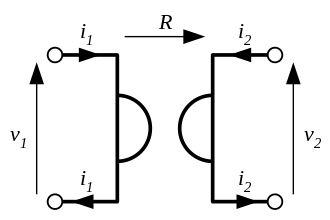
\includegraphics[width=0.7\textwidth]{gyratorsimb.png}
	\caption{Simbolo eléctrico del Gyrator.}
	\label{fig:gyrsimb}
\end{figure}
Realmente es implementado utilizando opamps, y uno de los usos mas populares es para la inversión de impedancias, permitiendo simular un inductor utilizando otros componentes.La configuración generalmente utilizada es la siguiente:
\begin{figure}[H]	
	\centering
	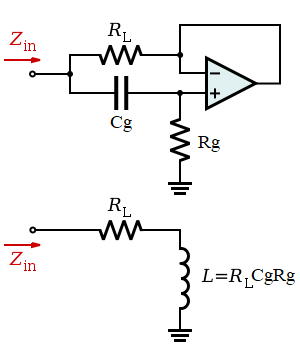
\includegraphics[width=0.5\textwidth]{gyrop.png}
	\caption{Equivalente del circuito Gyrator.}
	\label{fig:gyrop}
\end{figure}

%%%%%%%%%%%%%%%%%%%%%%%%%%%%%%%%%%%%%%%%%
\subsection{Calculo analítico.}
Utilizando el circuito de la figura (\ref{fig:gyrop}) se plantearon las siguientes ecuaciones:
\begin{align}   V_{Out} = V^- \label{eq:1}\end{align}
\begin{align} V_{Out} = A(s) \cdot (V^+-V^-)\label{eq:2}\end{align}
\begin{align} A(s)= \frac{A_0}{1+\frac{s}{\omega'}}\end{align}
\begin{align} I_{In}=\frac{V_{In}-V^-}{R_L}+\frac{V^+}{R_g}\end{align}
\begin{align} V^+=V_{In}\cdot \frac{R_g}{R_g+\frac{1}{sC_g}} \end{align}
primero observaremos que en utilizando (\ref{eq:1}) y (\ref{eq:2}) se llega a que 
\begin{align}V^- =V^+ \cdot \frac{A(s)}{A(s)+1} = V^+ \cdot \frac{A_0}{A_0+1+\frac{s}{\omega'}} \approx V^+ \cdot \frac{1}{1+\frac{s}{GBP}} \label{eq:desp}   \end{align}
Donde GBP es un parámetro propio del operacional y suele ser del orden de los MHz. Por lo tanto este termino sería desprecianle siempre que el rango de frecuencias en los cuales se trabaje sea menor a... \center \textcolor{red}{Obtener algun valor significativo}
, teniendo en cuenta esa aproximacion se pueden llegar a las siguientes expresiones:
\begin{align}H(s)= \frac{R_g}{R_g+\frac{1}{sC_g}} \end{align}


\begin{align}Z_{In}=\frac{R_LR_gC_gs+R_L}{sC_gR_L+1}\underset{C_gR_Ls << 1}{\approx}R_gC_gR_L \cdot s + R_g \end{align}

Bajo estos supuestos se puede considerar la impedancia de entrada como una bobina con 
\begin{align}  L=R_gC_gR_L  \ \ \ \ \ \  R_L=r_{coil} \label{eq:basicL1}\end{align}
\subsubsection{Gyrator vs Inductor}

\subsubsection{Impedancia de entrada.}

\subsubsection{Elección operacional.}

%%%%%%%%%%%%%%%%%%%%%%%%%%%%%%%%%%%%%%
 \flushleft
\subsection{Filtros de segundo orden.}
Los filtros a implemetar en este trabajo serán filtros de segundo orden siendo estos Low-Pass, High-Pass, Band-Pass y Band-Reject. Y tendran las siguientes especificaciones de diseño:
\begin{table}[H]
\begin{center}
\begin{tabular}{|c|c|c|c|}
\hline
\textbf{Tipo de Filtro} & \textbf{$f_p$ [Hz]} & \textbf{$f_a$ [Hz]} & \textbf{$f_c$ [Hz]} \\ \hline
\textbf{LP}             & 1000                & 3500                & \textbf{-}          \\ \hline
\textbf{HP}             & 10500               & 3000                & \textbf{-}          \\ \hline
\textbf{BP}             & -                   & -                   & 2000                \\ \hline
\textbf{BR}             & -                   & -                   & 3000                \\ \hline
\end{tabular}
\caption{Tabla de especificaciones.}
\label{tab:specs}
\end{center}
\end{table}
Para el caso de LP que tenga ganancia unitaria para la continua que tenga una ganancia mayor a -3dB para frecuencias menores a $f_p$ y menor a -10dB para frecuencais mayores a $f_a$. Para el HP se desea que tenga ganancia unitaria para valores de $f$ muy grandes, que tenga una ganancia mayor a -3dB para frecuencias mayores a $f_p$ y menor a -10dB para frecuencais menores a $f_a$
Algunos parametros que vale la pena recordar de filtros de segundo orden son:
\begin{table}[H]
\begin{center}
\begin{tabular}{c|cl}
$\omega_0$: & Frecuencia de corte del sistema en [$\frac{rad}{s}$] & =$\frac{1}{\sqrt{LC}}$         \\
$\xi$:      & Factor de Amortiguamiento del sistema.               & =$\frac{R\sqrt{C}}{2\sqrt{L}}$ \\
Q:          & Selectividad del sistema                             & =$\frac{1}{2\xi}$             
\end{tabular}
\end{center}
\caption{Parametros útiles.}
\label{tab:utils}
\end{table}

%%%%%%%%%%%%%%%%%%%%%%%%%%%%%%%%%%%%%%%%%%%%
\subsection{High Pass.}
\subsubsection{Circuito utilizando inductor.}
El circuito propuesto para realizar un filtro pasa altos clasicamente es el siguiente:

\begin{figure}[H]
\begin{center}
\begin{circuitikz}
	\node [](v2){};
	\draw (v2) node[label=left:$V_{In}$]{} to[short, o-] ++ (0.5,0) to[R, l = $R$]++ (1.5,0) to[C, l = $C$] ++ (2,0) to[open] ++(0,-2) node[ground](gnd){};
	\draw (gnd) to[L, l_= $L$] ++(0,2);
	\draw (v2) to[open] ++(4,0) to[short, -o] ++(1,0) node[label=right:$V_o$](){};
	\end{circuitikz}
	\caption{Filtro High-Pass básico.}
	\label{fig:basHP}
\end{center}
\end{figure}

Para este circuito es sumamente facil obtener la transferencia, basta con plantear un divisor resistivo, con lo cual se llega a:
\begin{align} 
H(s)=\frac{s^2LC+s\cdot r_{coil}C}{s^2LC+s\cdot(R+r_{coil})C+1}
\label{eq:HPL}
 \end{align}

\subsubsection{Circuito utilizando Gyrator.}
Para la implementación de este filtro utilizando un Gyrator dado a que este usualmente esta referenciado a tierra  se optó por el siguiente diseño:
\begin{figure}[H]	
	\centering
	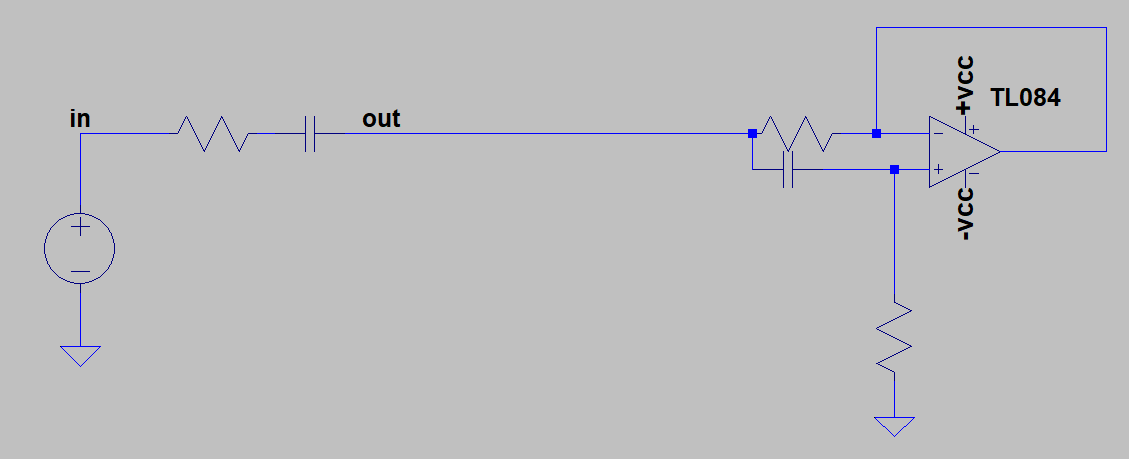
\includegraphics[width=0.7\textwidth]{gyrHP.PNG}
	\caption{Filtro High-Pass implementado con Gyrator.}
	\label{fig:gyrHP}
\end{figure}



Utilizando las siguientes ecuaciones se puede llegar a la expresión de la transferencia:
\begin{align}V^- = V_{o'}\end{align}
\begin{align}V_{o'} = A(s)\cdot (V^+-V^-)\end{align}
\begin{align}\frac{V_o-V_i}{R+\frac{1}{sC}} = \frac{V^+-V_o}{R_L}+(V^+-V_o)\cdot sC_g\end{align}
\begin{align}\frac{-V^+}{R_g}=(V^+-V_o)\cdot sC_g\end{align}
%\begin{align}\end{align}
\begin{align} H(s) = \frac{C R_L s \left(C_g R_g s + 1\right)}{C C_g R R_L s^{2} + C C_g R_g R_L s^{2} + C R s + C R_L s + C_g R_L s + 1}\label{eq:transgyrHP}\end{align}\footnote{Teniendo en cuenta que se despreció el término (\ref{eq:desp}) de (\ref{eq:transgyrHP})}
Luego teniendo en cuenta (\ref{eq:basicL1}) y tomando que
\begin{align} C_gR_LRC<<LC \implies R<<R_g \end{align}
La transferencia  se puede expresar como:
 \begin{align} H(s) = \frac{LC\cdot s^2+Cr_{coil}\cdot s}{s^2 \cdot (LC)+s\cdot C(R+r_{coil})+1}\label{eq:transgyrHPfinal} 
\end{align}
Vale la pena destacar que (\ref{eq:HPL}) y (\ref{eq:transgyrHPfinal}) son iguales.
Es de utilidad recordar las aproximiaciones utilizadas hasta ahora:
\begin{align}  \frac{1}{1+\frac{s}{GBP}}\approx 1  \ \ \ R<<R_g \ \ \ C_gR_Ls << 1 \label{eq:basicL2}\end{align}
\subsubsection{Comparación de modelos.}
\subsubsection{PCB.}
\subsubsection{Respuesta en frecuencia.}
\subsubsection{Analisis de resultados.}

\newpage
%%%%%%%%%%%%%%%%%%%%%%%%%%%%%%%%%%%%%%%%%%%%
\subsection{Low Pass.}
\subsubsection{Circuito utilizando inductor.}
El circuito propuesto para realizar un filtro pasa bajos clasicamente es el siguiente:

\begin{figure}[H]
\begin{center}
\begin{circuitikz}
	\node [](v2){};
	\draw (v2) node[label=left:$V_{In}$]{} to[short, o-] ++ (0.5,0) to[R, l = $R$]++ (1.5,0) to[L, l = $L$] ++ (2,0) to[open] ++(0,-2) node[ground](gnd){};
	\draw (gnd) to[C, l_= $C$] ++(0,2);
	\draw (v2) to[open] ++(4,0) to[short, -o] ++(1,0) node[label=right:$V_o$](){};
	\end{circuitikz}
	\caption{Filtro Low-Pass básico.}
	\label{fig:basLP}
\end{center}
\end{figure}
Obteniendo la transferencia del circuito se obtiene:
\begin{align}
H(s)=\frac{1}{s^2\cdot LC+s\cdot C(R+r_{coil})+1}
\label{eq:LPL}
\end{align}
La cual verifica ser un pasabajos.
\subsubsection{Circuito utilizando Gyrator.}
El gyrator tiene la particularidad de que debe estar referenciado a tierra para funcionar como tal, en este caso lo utilizaremos "flotando" para realizar el filtro pasa bajos, el circuito propuesto fue el siguiente.
\begin{figure}[H]	
	\centering
	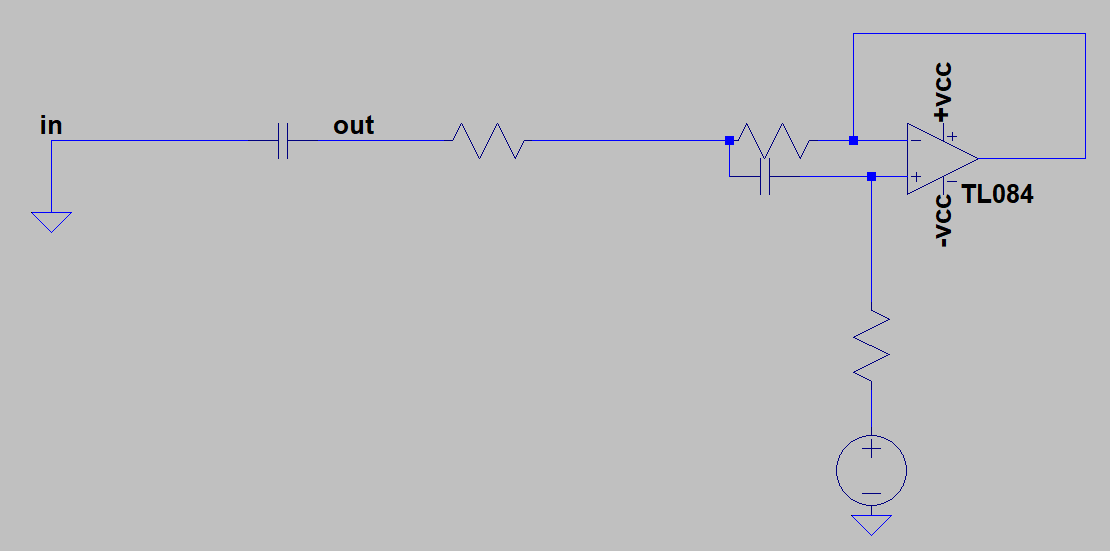
\includegraphics[width=0.7\textwidth]{gyrLP.PNG}
	\caption{Filtro Low-Pass implementado con Gyrator.}
	\label{fig:gyrLP}
\end{figure}

Utilizando las siguientes ecuaciones se puede llegar a la expresión de la transferencia:
\begin{align}V^- = V_{o'}\end{align}
\begin{align}V_{o'} = A(s)\cdot (V^+-V^-)\end{align}
\begin{align}\frac{V_{In}-V^+}{R_g}=(V^+-V_n)\cdot s C_g\end{align}
\begin{align}V_{out}\cdot s C=\frac{V_{n}-V_{out}}{R}\end{align}
\begin{align}\frac{V_{n}-V_{out}}{R}=\frac{V^--V_n}{R_L} +(V^+-V_n)\cdot s C_g\end{align}
%\begin{align}\end{align}
Operando se obtiene:
\begin{equation} H(s)= \frac{\left(C_g R_L s + 1\right)}{C C_g R R_L s^{2} + C C_g R_g R_L s^{2} + C R s + C R_L s + C_g R_L s + 1}
\end{equation}
Utilizando (\ref{eq:basicL1}) y (\ref{eq:basicL2}) se llega a que:
\begin{equation} H(s)= \frac{1}{C L s^{2} + s\cdot C (R+r_{coil}) + 1}
\label{eq:LPG}
\end{equation}
Vale la pena destacar que (\ref{eq:LPL}) y (\ref{eq:LPG}) son iguales.
\subsubsection{Comparación de modelos.}
\subsubsection{PCB.}
\subsubsection{Respuesta en frecuencia.}
\subsubsection{Analisis de resultados.}
\newpage
%%%%%%%%%%%%%%%%%%%%%%%%%%%%%%%%%%%%%%%%%%%%
\subsection{Band Pass.}
\subsubsection{Circuito utilizando inductor.}
El circuito propuesto para realizar un filtro pasa banda clasicamente es el siguiente:

\begin{figure}[H]
\begin{center}
\begin{circuitikz}
	\node [](v2){};
	\draw (v2) node[label=left:$V_{In}$]{} to[short, o-] ++ (0.5,0) to[R, l = $R$]++ (2.5,0)  to[open] ++(0,-2) node[ground](gnd){};
	\draw (gnd) to[C, l_= $C$] ++(0,2);
	\draw(5,-2) node[ground](gnd2){};
	\draw (gnd2) to[L, l_= $L$] ++(0,2);

	\draw (v2) to[open] ++(3,0) to[short, -o] ++(3,0) node[label=right:$V_o$](){};
	\end{circuitikz}
	\caption{Filtro Band-Pass básico.}
	\label{fig:basBP}
\end{center}
\end{figure}
Operando en el circuito se obtiene:
\begin{align}H(s)=\frac{s\cdot \frac{L}{R}+\frac{r_{coil}}{R}}{s^2 LC+s\cdot (Cr_{coil}+\frac{L}{R})+1+\frac{r_{coil}}{R}}
	\label{eq:BPL}
\end{align}
%\begin{align}\end{align}
\subsubsection{Circuito utilizando Gyrator.}
El circuito propuesto para el filtro Band-Pass es identico a la figura (\ref{fig:basBP}) con la singularidad que intercambiaremos el inductor por un gyrator de la siguiente manera.
\begin{figure}[H]	
	\centering
	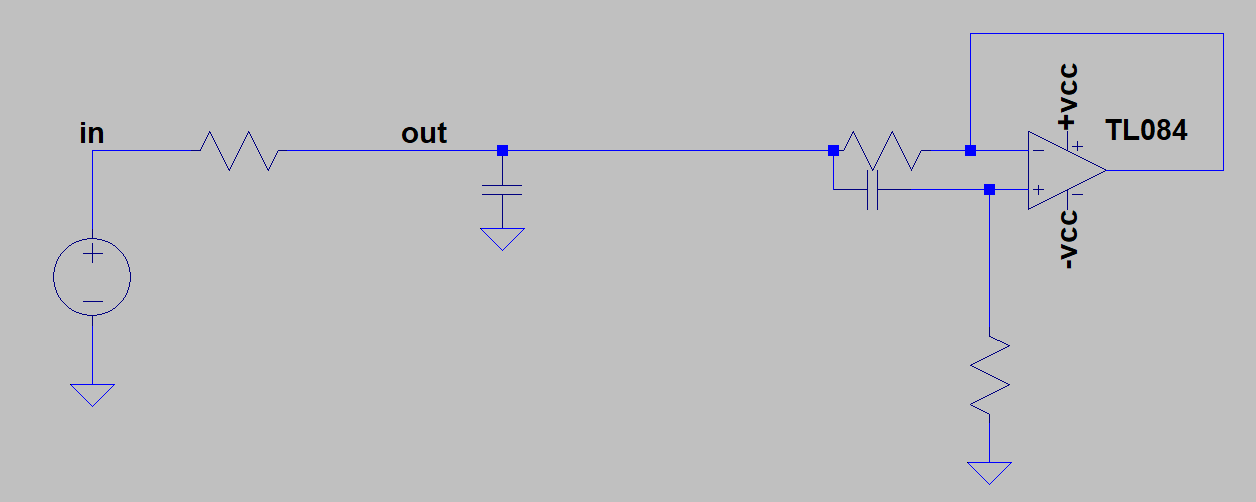
\includegraphics[width=0.7\textwidth]{gyrBP.PNG}
	\caption{Filtro Band-Pass implementado con Gyrator.}
	\label{fig:gyrBP}
\end{figure}
Para resolver el circuito se plantearon la siguientes ecuaciones:
\begin{align}V^- = V_{o'}\end{align}
\begin{align}V_{o'} = A(s)\cdot (V^+-V^-)\end{align}
\begin{align} -\frac{V^+}{R_g}=(V^+-V_{out})\cdot sC_g \end{align}
\begin{align}  V_{out}\cdot sC= \frac{V^--V_{out}}{R_L}+\frac{V_{in}-V_{out}}{R}-\frac{V_{out}}{R_g+\frac{1}{sC_g}}\end{align}
Se llega a que:
\begin{align}H(s)=\frac{R_{L} \left(C_{g} R_{g} s + 1\right)}{C C_{g} R R_{L} R_{g} s^{2} + C R R_{L} s + C_{g} R R_{L} s + C_{g} R_{L} R_{g} s + R + R_{L}}
\end{align}
Teniendo en cuenta (\ref{eq:basicL1}) y (\ref{eq:basicL2}) se obtiene:
\begin{align}H(s)=\frac{s\frac{L}{R}+\frac{r_{coil}}{R}}{s^2\cdot LC +s \cdot (Cr_{coil}+\frac{L}{R})+1+\frac{r_{coil}}{R}}
\label{eq:BPG}
\end{align}
Vale la pena destacar que (\ref{eq:BPL}) y (\ref{eq:BPG}) son iguales.
\subsubsection{Comparación de modelos.}
\subsubsection{PCB.}
\subsubsection{Respuesta en frecuencia.}
\subsubsection{Analisis de resultados.}
\newpage
%%%%%%%%%%%%%%%%%%%%%%%%%%%%%%%%%%%%%%%%%%%%
\subsection{Band Reject.}
\subsubsection{Circuito utilizando inductor.}
El circuito propuesto para realizar un filtro rechaza banda clasicamente es el siguiente:
\begin{figure}[H]
\begin{center}
\begin{circuitikz}
	\node [](v2){};
	\draw (v2) node[label=left:$V_{In}$]{} to[short, o-] ++ (0.5,0) to[R, l = $R$]++ (1.5,0) to[L, l = $L$] ++ (0,-2) to[open](2,-4) node[ground](gnd){};
	\draw (gnd) to[C, l_= $C$] ++(0,2);
	\draw (v2) to[open] ++(2,0) to[short, -o] ++(1,0) node[label=right:$V_o$](){};
	\end{circuitikz}
	\caption{Filtro Band-Reject básico.}
	\label{fig:basBR}
\end{center}
\end{figure}
Al cual le corresponde una transferencia de la forma:
\begin{align} H(s)=\frac{s^2\cdot LC+s\cdot r_{coil}C+1}{s^2\cdot LC+s\cdot (RC+r_{coil}C)+1}
\label{eq:BRL}
\end{align}
\subsubsection{Circuito utilizando Gyrator.}
\begin{figure}[H]	
	\centering
	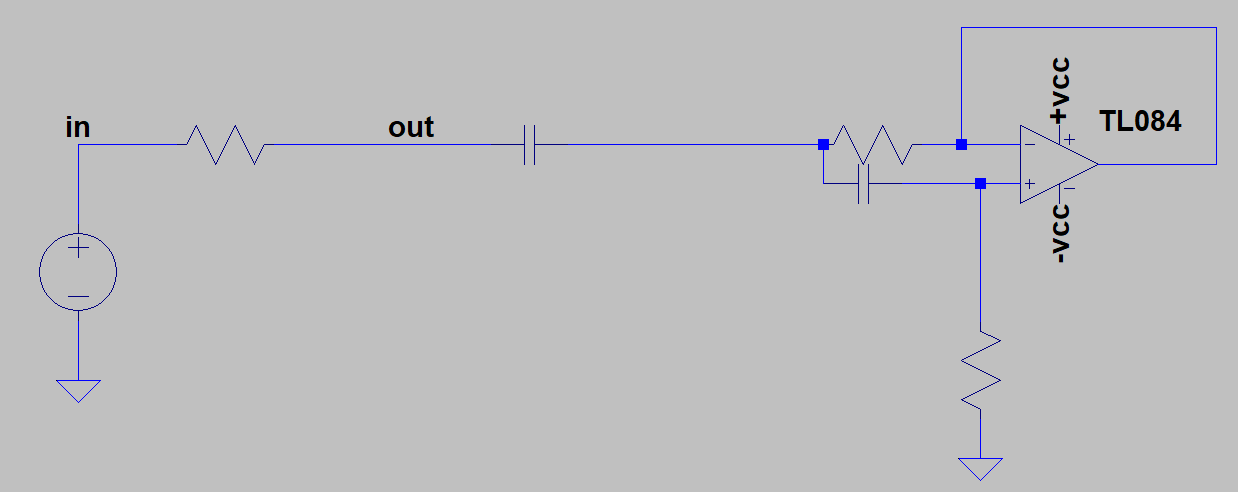
\includegraphics[width=0.7\textwidth]{gyrBR.PNG}
	\caption{Filtro Band-Reject implementado con Gyrator.}
	\label{fig:gyrBR}
\end{figure}
Luego se procedió a analizar el circuito para sacar la función transferencia:
\begin{align}V^- = V_{o'}\end{align}
\begin{align}V_{o'} = A(s)\cdot (V^+-V^-)\end{align}
\begin{align}\frac{V_{out}-V_{in}}{R}=(V_n-V_{out})\cdot sC\end{align}
\begin{align}(V_n-V_{out})\cdot sC = \frac{-V_n}{R_g+\frac{1}{sC_g}}+\frac{V^--V_n}{R_L}\end{align}
\begin{align}\frac{-V^+}{R_g}=(V^+-V_n)\cdot sC_g\end{align}
Se llega a :
\begin{align}  H(s)=\frac{C C_{g} R_{L} R_{g} s^{2} + C R_{L} s + C_{g} R_{L} s + 1}{C C_{g} R R_{L} s^{2} + C C_{g} R_{L} R_{g} s^{2} + C R s + C R_{L} s + C_{g} R_{L} s + 1} \end{align}
Teniendo en cuenta (\ref{eq:basicL1}) y (\ref{eq:basicL2}) se obtiene:
\begin{align}  H(s)=\frac{ s^{2}\cdot  LC + s \cdot  C r_{coil} + 1}{ s^{2}\cdot LC + s\cdot (C R+Cr_{coil}) + 1} 
\label{eq:BRG}
\end{align}
\subsubsection{Comparación de modelos.}
\subsubsection{PCB.}
\subsubsection{Respuesta en frecuencia.}
\subsubsection{Analisis de resultados.}

\end{document}
%\begin{align}\end{align}